%\documentclass[5p,times]{elsarticle}
\documentclass[11pt,review,times]{article}
%\documentclass[11pt,preprint,times]{elsarticle}

%%%%%%%%%%%%%%%%%%%%%%%%%%%%%%%%%%%%%%%%%%%%%%%%%%%%%%%%%%%%%%%%%
%	Loading packages
%%%%%%%%%%%%%%%%%%%%%%%%%%%%%%%%%%%%%%%%%%%%%%%%%%%%%%%%%%%%%%%%%
\usepackage[english]{babel}
\usepackage[utf8]{inputenc}
\usepackage[T1]{fontenc}
\usepackage{graphicx}
\usepackage{amsfonts}
\usepackage{placeins} % For /Floatbarrier
\usepackage{array,booktabs}
\usepackage{url} % For better linebreaks of URLs
\usepackage{float}

\usepackage[list-units = single,range-units = single]{siunitx}
\sisetup{separate-uncertainty}

\usepackage{caption}
\usepackage{subcaption}
\usepackage{upgreek}
\usepackage[inline]{enumitem}
\usepackage{chemformula}
%\usepackage{mathrsfs}
%\usepackage{wasysym}


% Packages for tikz
\usepackage{tikz}
\usepackage{pgf}
\usepackage{pgfplots}
\usepackage{pgfplotstable}
	\pgfplotstableset{col sep=comma} % call once in your preamble if all your tables use commas as column separator
	\pgfplotstableset{search path={datafiles}} % Put .csv files in /datafiles or the root folder
\usetikzlibrary{3d}
\usetikzlibrary{calc}
\usetikzlibrary{decorations.pathmorphing} % Pour obtenir des lignes de coupes aléatoires
\usetikzlibrary{arrows}
\usetikzlibrary{arrows.meta,shapes,positioning,shadows,trees,decorations.pathmorphing}
\usetikzlibrary{external}
\tikzexternalize[prefix=TikzPictures/]

\usepackage[sort&compress]{natbib}
\setcitestyle{numbers,square,comma}

\newcolumntype{M}[1]{>{\centering\arraybackslash}m{#1}} % Define a column style "M" (verticaly centered by m) and horizontaly

% Hyperref and parameters of PDF
\usepackage[hidelinks]{hyperref}
\hypersetup{
	pdftitle = {Resistance Welding of Thermoplastic Composites with a Nanocomposite Heating Element},
    pdfauthor = {David Brassard, Martine Dubé, Jason R Tavares},
	pdfkeywords={carbon nanotube, thermal conductivity, polymer, nanocomposite, heating element, Joule heating, electrical conductivity, Finite element analysis, composite, thermoplastic},
	pdfsubject={Resistance Welding of Thermoplastic Composites with a Nanocomposite Heating Element}
}

\graphicspath{{Figures/}}	% Root directory of the pictures 

%%%%%%%%%%%%%%%%%%%%%%%%%%%%%%%%%%%%%%%%%%%%%%%%%%%%%%%%%%%%%%%%%
%	Main document
%%%%%%%%%%%%%%%%%%%%%%%%%%%%%%%%%%%%%%%%%%%%%%%%%%%%%%%%%%%%%%%%%
\begin{document}
\hyphenation{COMSOL na-no-com-po-si-te na-no-com-po-si-tes}


\title{Supplementary Information for the Article : Resistance Welding of Thermoplastic Composites with a Nanocomposite Heating Element}
\author{David~Brassard, Martine~Dubé, Jason~R.~Tavares}

\maketitle


%%%%%%%%%%%%%%%%%%%%%%%%%%%%%%%%%%%%%%%%%%%%%%%%%%%%%%%%%%%%%%%%%
							\section{Supplementary Information}
%%%%%%%%%%%%%%%%%%%%%%%%%%%%%%%%%%%%%%%%%%%%%%%%%%%%%%%%%%%%%%%%%

This document contain supplementary information in regard to the article titled "Resistance Welding of Thermoplastic Composites with a Nanocomposite Heating Element" published in Composites Part B: Engineering. 

%%%%%%%%%%%%%%%%%%%%%%%%%%%%%%%%%%%%%%%%%%%%%%%%%%%%%%%%%%%%%%
\subsection{Continuum Micromechanic Simulations}
%%%%%%%%%%%%%%%%%%%%%%%%%%%%%%%%%%%%%%%%%%%%%%%%%%%%%%%%%%%%%%

In the early phase of the nanocomposite heating elements development, finite element models were developed using COMSOL Mul\-ti\-phy\-sics\-\textregistered \ to verify that the polymer would not undergo thermal degradation and to evaluate the contribution of the three main heating mechanisms inside the nanocomposite heating element (i.e. Joule heating of MWCNTs, from the concentration of charges at the contact points between MWCNTs and of the matrix between MWCNTs).  
A set of three continuum micromechanic models presenting different contact topologies were used to asses the relative contribution of each heating mechanism to the global heating phenomena within a conductive nanocomposite. 
Representative elementary volumes (REV) in which the MWCNTs represented 1\% of the total mass were used in these models (Fig. \ref{fig:geometry}). 

\begin{figure}[htb]
	\center
	\begin{subfigure}{0.28\textwidth}
		\center
		\captionsetup{width=0.9\textwidth}
		%\resizebox{35mm}{!}{
		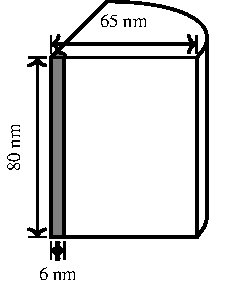
\includegraphics[width=\textwidth]{geometry_axisymmetric}
		%\tikzsetnextfilename{geometry_axisymmetric}
		%%\shorthandoff{:!}

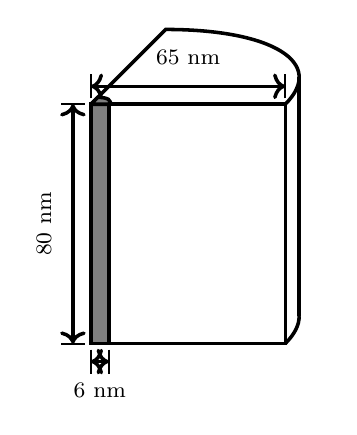
\begin{tikzpicture}[scale=0.038]

%%%%%%%%%%%%%%%%%%%%%%
%%%	 Def géométrie  %%%
%%%%%%%%%%%%%%%%%%%%%%

\def \rayonun{6}
\def \rayondeux{65}
\def \vspace{2}
\def \lignecote{8}
\def \hauteur{80}
\def \anglearc{111.5}

%%%%%%%%%%%%%%%%%%%%%%
%%%	   Def style    %%%
%%%%%%%%%%%%%%%%%%%%%%

\def \heavy{0.045cm}
\def \light{0.025cm}

%%%%%%%%%%%%%%%%%%%%%%
%%%	    Calculs     %%%
%%%%%%%%%%%%%%%%%%%%%%

\pgfmathsetmacro{\sinangle}{sin(\anglearc)}
\pgfmathsetmacro{\cosangle}{cos(\anglearc)}

%%%%%%%%%%%%%%%%%%%%%%
%%%	    Dessin      %%%
%%%%%%%%%%%%%%%%%%%%%%

\draw[line width=\heavy] (\rayonun,0) rectangle (\rayondeux,\hauteur);
\draw[line width=\heavy, fill=gray] (0,0) rectangle (\rayonun,\hauteur);
%\draw[line width=\heavy] \draw (0,0,0) arc (0:45:1) ;

% On se positionne sur un plan à une hauteur de 80 (\hauteur)
\begin{scope}[canvas is zx plane at y=\hauteur]
	% On dessine le quart de cercle extérieur
	\draw[line width=\heavy] (0,\rayondeux) arc (90:180:\rayondeux) -- (0,0);
	% On dessine le quart de cercle du nanotube
	\draw[line width=\heavy, fill=gray] (0,0) -- (0,\rayonun) arc (90:180:\rayonun) -- (0,0);
\end{scope}

% On se positionne sur un plan à une hauteur de 0
\begin{scope}[canvas is zx plane at y=0]
	% On trace le cercle jusqu'à l'angle \anglearc trouvé itérativement
	\draw[line width=\heavy] (0,\rayondeux) arc (90:\anglearc:\rayondeux);
\end{scope}

% Ligne du côté du cylindre
\draw[line width=\heavy] (\sinangle*\rayondeux,0,\cosangle*\rayondeux) -- +(0,\hauteur,0);

%%%%%%%%%%%%%%%%%%%%%%
%%%	    Cotation    %%%
%%%%%%%%%%%%%%%%%%%%%%

% On dessine la ligne de cote pour la nanotube
\draw[line width=\light] (0,-\vspace) -- + (0,-\lignecote);
\draw[line width=\light] (\rayonun,-\vspace) -- + (0,-\lignecote);
\draw[<->,line width=\heavy] (0,-\vspace-0.5*\lignecote) -- + (\rayonun,0);

\node[anchor=north] (A) at (0.5*\rayonun , -\vspace-\lignecote) {\footnotesize \rayonun \ nm};

% On dessine la ligne de cote pour la hauteur
\draw[line width=\light] (-\vspace,0) -- + (-\lignecote,0);
\draw[line width=\light] (-\vspace,\hauteur) -- + (-\lignecote,0);
\draw[<->,line width=\heavy] (-\vspace-0.5*\lignecote,0) -- + (0,\hauteur);

\node[anchor=south, rotate=90] (A) at (-\vspace-\lignecote,0.5*\hauteur ) {\footnotesize \hauteur \ nm};

% On dessine la ligne de cote pour le diamètre du modèle
\draw[line width=\light] (0,\hauteur+\vspace) -- + (0,\lignecote);
\draw[line width=\light] (\rayondeux,\hauteur+\vspace) -- + (0,\lignecote);
\draw[<->,line width=\heavy] (0,\hauteur+\vspace+0.5*\lignecote) -- + (\rayondeux,0);

\node[anchor=south] (A) at (0.5*\rayondeux , \hauteur+\vspace+\lignecote) {\footnotesize \rayondeux \ nm};

%%%%%%%%%%%%%%%%%%%%%%%%%%%%%%%%%%%%%%%%%

\end{tikzpicture}

%\shorthandon{:!}
		%}
		\caption{Quarter view of the revolved 2D axisymmetric FEM simulating the Joule heating within a MWCNT}
		\label{fig:geometry_axisymmetric}
	\end{subfigure}%
	\begin{subfigure}{0.44\textwidth}
		\center
		\captionsetup{width=0.9\textwidth}
		%\resizebox{65mm}{!}{
		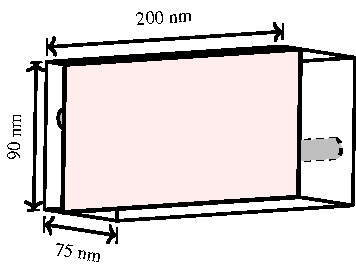
\includegraphics[width=\textwidth]{geometry_3D}
		%\tikzsetnextfilename{geometry_3D}
		%%\shorthandoff{:!}

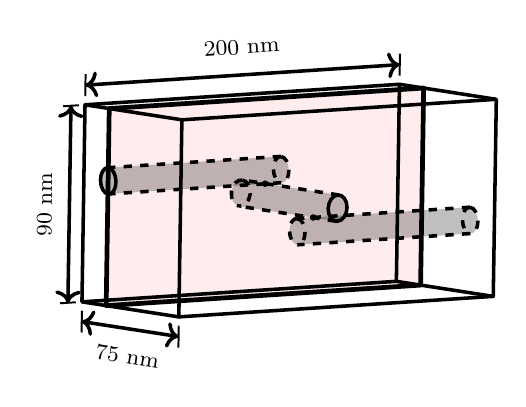
\begin{tikzpicture}[scale=0.02,
								x  = {(0.99788,0.065079)},
                    		y  = {(0.021693,1.38835)},
                    		z  = {(-0.824336,0.130158)},]

%%%%%%%%%%%%%%%%%%%%%%
%%%	 Def géométrie  %%%
%%%%%%%%%%%%%%%%%%%%%%

\def \dia{6} %La variable dia contient en fait le rayon des tubes au lieu du diamètre
\def \epaisseur{75}
\def \hauteur{90}
\def \longueur{200}

\def \angle{88.0}

\def \vspace{4}
\def \lignecote{10}
\def \anglearc{111.5}

\def \colplan{red!7}
\def \coltube{gray!50}

\def \dotsize{60pt}

\coordinate (A) at (0,0,0);
\coordinate (B) at (0,0,\epaisseur);
\coordinate (C) at (0,\hauteur,\epaisseur);
\coordinate (D) at (0,\hauteur,0);
\coordinate (E) at (-\longueur,0,0);
\coordinate (F) at (-\longueur,0,\epaisseur);
\coordinate (G) at (-\longueur,\hauteur,\epaisseur);
\coordinate (H) at (-\longueur,\hauteur,0);

\coordinate (W) at (0,0,0.75*\epaisseur);
\coordinate (X) at (0,\hauteur,0.75*\epaisseur);
\coordinate (Y) at (-\longueur,\hauteur,0.75*\epaisseur);
\coordinate (Z) at (-\longueur,0,0.75*\epaisseur);


%%%%%%%%%%%%%%%%%%%%%%
%%%	   Def style    %%%
%%%%%%%%%%%%%%%%%%%%%%

\def \heavy{0.045cm}
\def \light{0.025cm}
\def \reallyheavy{0.06cm}

%Modification du monde de transparence pour mélanger les couleurs superposées
\begin{scope}[blend mode=multiply]

%%%%%%%%%%%%%%%%%%%%%%
%%%	    Calculs     %%%
%%%%%%%%%%%%%%%%%%%%%%

\pgfmathsetmacro{\sinangle}{sin(\anglearc)}
\pgfmathsetmacro{\cosangle}{cos(\anglearc)}

\pgfmathsetmacro{\sinangledeux}{sin(\angle)}
\pgfmathsetmacro{\cosangledeux}{cos(\angle)}

%%%%%%%%%%%%%%%%%%%%%%
%%%	 Dessin du cube %%%
%%%%%%%%%%%%%%%%%%%%%%

\draw[line width=\heavy, line join=round] (A) -- (B) -- (C) --(D) -- cycle;
\draw[line width=\heavy, line join=round] (E) -- (F) -- (G) --(H) -- cycle;
\draw[line width=\heavy, line join=round] (D) -- (H);
\draw[line width=\heavy, line join=round] (G) -- (C);
\draw[line width=\heavy, line join=round] (A) -- (E);
\draw[line width=\heavy, line join=round] (F) -- (B);


%%%%%%%%%%%%%%%%%%%%%%%%%%%%%%%%%%%%
%%% Dessin du nanotube du centre %%%
%%%%%%%%%%%%%%%%%%%%%%%%%%%%%%%%%%%%

%Trouver les distances projetées en x et y pour un vecteur unitaire pour chaque axe
\path (1,0,0);
\pgfgetlastxy{\cylxx}{\cylxy}
\path (0,1,0);
\pgfgetlastxy{\cylyx}{\cylyy}
\path (0,0,1);
\pgfgetlastxy{\cylzx}{\cylzy}

%Calculs
\pgfmathsetmacro{\cylt}{(\cylzy * \cylyx - \cylzx * \cylyy)/ (\cylzy * \cylxx - \cylzx * \cylxy)}
\pgfmathsetmacro{\ang}{atan(\cylt)}
\pgfmathsetmacro{\ct}{1/sqrt(1 + (\cylt)^2)}
\pgfmathsetmacro{\st}{\cylt * \ct}

%\node[anchor=north] (A) at (0,-30,0) {\large xx \cylxx};
%\node[anchor=north] (A) at (0,-40,0) {\large xy \cylxy};
%\node[anchor=north] (A) at (0,-50,0) {\large yx \cylyx};
%\node[anchor=north] (A) at (0,-60,0) {\large yy \cylyy};
%\node[anchor=north] (A) at (0,-70,0) {\large zx \cylzx};
%\node[anchor=north] (A) at (0,-80,0) {\large zy \cylzy};
%\node[anchor=north] (A) at (0,-90,0) {\large \cylt};
%\node[anchor=north] (A) at (0,-100,0) {\large \ang};
%\node[anchor=north] (A) at (0,-110,0) {\large \ct};
%\node[anchor=north] (A) at (0,-120,0) {\large \st};

%\draw[line width=0.45, line join=round] (A) -- (H);

%Surface extérieure du cylindre
\fill[\coltube] (-0.5*\longueur+\dia*\ct,0.5*\hauteur+\dia*\st,\epaisseur) -> ++(0,0,-\epaisseur) arc[start angle=\ang,delta angle=180,radius=\dia] -- ++(0,0,\epaisseur) arc[start angle=\ang+180,delta angle=-180,radius=\dia];

%Lignes des côtés
\begin{scope}[every path/.style={line width=\heavy}]

	%Cercle du devant
	\draw[fill=\coltube] (-0.5*\longueur,0.5*\hauteur,0) circle[radius=\dia];

	%Ligne des côtés
	\draw[dashed] (-0.5*\longueur+\dia*\ct,0.5*\hauteur+\dia*\st,0) -- ++(0,0,\epaisseur);
	\draw[dashed] (-0.5*\longueur-\dia*\ct,0.5*\hauteur-\dia*\st,0) -- ++(0,0,\epaisseur);

	%Cercle arrière
	\draw[dashed] (-0.5*\longueur+\dia*\ct,0.5*\hauteur+\dia*\st,\epaisseur) arc[start angle=\ang,delta angle=180,radius=\dia];
	\draw[dashed] (-0.5*\longueur+\dia*\ct,0.5*\hauteur+\dia*\st,\epaisseur) arc[start angle=\ang,delta angle=-180,radius=\dia];
	
\end{scope}

%\draw (-0.5*\longueur,.5*\hauteur,0) -- (-0.5*\longueur,.5*\hauteur,\epaisseur);

%%%%%%%%%%%%%%%%%%%%%%%%%%%%%%%%%%%%
%%% Dessin du nanotube de droite %%%
%%%%%%%%%%%%%%%%%%%%%%%%%%%%%%%%%%%%

\begin{scope}[canvas is zy plane at x=0]
	\draw[line width=\heavy, dashed] (0.25*\epaisseur,0.5*\hauteur-2*\dia) ++(\angle:\dia) arc[start angle=\angle,delta angle=-180,radius=\dia];
	\draw[line width=\heavy, dashed, fill=\coltube] (0.25*\epaisseur,0.5*\hauteur-2*\dia) ++(\angle:\dia) arc[start angle=\angle,delta angle=180,radius=\dia];
\end{scope}


\begin{scope}[canvas is zy plane at x=-0.55*\longueur]
	\draw[line width=\heavy, dashed, fill=\coltube] (0.25*\epaisseur,0.5*\hauteur-2*\dia) ++(\angle:\dia) arc[start angle=\angle,delta angle=-180,radius=\dia];
	\draw[line width=\heavy, dashed] (0.25*\epaisseur,0.5*\hauteur-2*\dia) ++(\angle:\dia) arc[start angle=\angle,delta angle=180,radius=\dia];
\end{scope}


\draw[line width=\heavy, dashed] (0,0.5*\hauteur-2*\dia+\dia*\sinangledeux,0.25*\epaisseur+\dia*\cosangledeux) -- ++(-0.55*\longueur,0,0);	

\draw[line width=\heavy, dashed] (0,0.5*\hauteur-2*\dia-\dia*\sinangledeux,0.25*\epaisseur-\dia*\cosangledeux) -- ++(-0.55*\longueur,0,0);	

\fill[\coltube] (0,0.5*\hauteur-2*\dia+\dia*\sinangledeux,0.25*\epaisseur+\dia*\cosangledeux) -- ++(-0.55*\longueur,0,0) -- ++(0,-2*\dia*\sinangledeux,-2*\dia*\cosangledeux)-- ++(0.55*\longueur,0,0) -- cycle;

%\draw (0,0.5*\hauteur-\dia,\epaisseur*0.25) -- ++(-0.55*\longueur,0,0);


%%%%%%%%%%%%%%%%%%%%%%%%%%%%%%%%%%%%
%%% Dessin du nanotube de gauche %%%
%%%%%%%%%%%%%%%%%%%%%%%%%%%%%%%%%%%%


\begin{scope}[canvas is zy plane at x=-\longueur]
	\draw[line width=\heavy, fill=\coltube] (0.75*\epaisseur,0.5*\hauteur+2*\dia) ++(\angle:\dia) arc[start angle=\angle,delta angle=-180,radius=\dia];
	\draw[line width=\heavy] (0.75*\epaisseur,0.5*\hauteur+2*\dia) ++(\angle:\dia) arc[start angle=\angle,delta angle=180,radius=\dia];
\end{scope}

\begin{scope}[canvas is zy plane at x=-0.45*\longueur]
	\draw[line width=\heavy, dashed] (0.75*\epaisseur,0.5*\hauteur+2*\dia) ++(\angle:\dia) arc[start angle=\angle,delta angle=-180,radius=\dia];
	\draw[line width=\heavy, dashed, fill=\coltube] (0.75*\epaisseur,0.5*\hauteur+2*\dia) ++(\angle:\dia) arc[start angle=\angle,delta angle=180,radius=\dia];
\end{scope}

\draw[line width=\heavy, dashed] (-0.45*\longueur,0.5*\hauteur+2*\dia+\dia*\sinangledeux,0.75*\epaisseur+\dia*\cosangledeux) -- ++(-0.55*\longueur,0,0);	

\draw[line width=\heavy, dashed] (-0.45*\longueur,0.5*\hauteur+2*\dia-\dia*\sinangledeux,0.75*\epaisseur-\dia*\cosangledeux) -- ++(-0.55*\longueur,0,0);	

\fill[\coltube] (-0.45*\longueur,0.5*\hauteur+2*\dia+\dia*\sinangledeux,0.75*\epaisseur+\dia*\cosangledeux) -- ++(-0.55*\longueur,0,0) -- ++(0,-2*\dia*\sinangledeux,-2*\dia*\cosangledeux)-- ++(0.55*\longueur,0,0) -- cycle;

%%%%%%%%%%%%%%%%%%%%%%%%%%%%%%%%%%%%
%%% Dessin des points de contact %%%
%%%%%%%%%%%%%%%%%%%%%%%%%%%%%%%%%%%%

\fill [black] (-0.5*\longueur,0.5*\hauteur-\dia,0.25*\epaisseur) circle (\dotsize);
\fill [black] (-0.5*\longueur,0.5*\hauteur+\dia,0.75*\epaisseur) circle (\dotsize);

%%%%%%%%%%%%%%%%%%%%%%%%%%%%%%%%%%%%
%%% Dessin du plan de decoupe    %%%
%%%%%%%%%%%%%%%%%%%%%%%%%%%%%%%%%%%%

\draw[line width=\reallyheavy, line join=round, fill=\colplan] (W) -- (X) -- (Y) --(Z) -- cycle;

%%%%%%%%%%%%%%%%%%%%%%
%%%	    Cotation    %%%
%%%%%%%%%%%%%%%%%%%%%%

%Calcul des angles de rotation pour les cotes
\pgfmathsetmacro{\rotx}{ atan( \cylxy / \cylxx) }
\pgfmathsetmacro{\roty}{ atan( \cylyx / \cylyy) }
\pgfmathsetmacro{\rotz}{ atan( \cylzy / \cylzx) }

% On dessine la ligne de cote pour la longueur
\draw[line width=\light] (-\longueur,\vspace+\hauteur,\epaisseur) -- + (0,\lignecote,0);
\draw[line width=\light] (0,\vspace+\hauteur,\epaisseur) -- + (0,\lignecote,0);
\draw[<->,line width=\heavy] (-\longueur,+\vspace+\hauteur+0.5*\lignecote,\epaisseur) -- + (\longueur,0,0);

\node[anchor=south, rotate=\rotx] (C) at (-0.5*\longueur,\hauteur+\vspace+\lignecote,\epaisseur ) {\footnotesize \longueur \ nm};

% On dessine la ligne de cote pour la hauteur
\draw[line width=\light] (-\longueur-\vspace,0,\epaisseur) -- + (-\lignecote,0,0);
\draw[line width=\light] (-\longueur-\vspace,\hauteur,\epaisseur) -- + (-\lignecote,0);
\draw[<->,line width=\heavy] (-\longueur-\vspace-0.5*\lignecote,0,\epaisseur) -- + (0,\hauteur);

\node[anchor=south, rotate=90-\roty] (C) at (-\longueur-\vspace-\lignecote,0.5*\hauteur,\epaisseur ) {\footnotesize \hauteur \ nm};

% On dessine la ligne de cote pour l'épaisseur
\draw[line width=\light] (-\longueur,-\vspace,\epaisseur) -- + (0,-\lignecote,0);
\draw[line width=\light] (-\longueur,-\vspace,0) -- + (0,-\lignecote,0);
\draw[<->,line width=\heavy] (-\longueur,-\vspace-0.5*\lignecote,\epaisseur) -- + (0,0,-\epaisseur);

\node[anchor=north, rotate=\rotz] (C) at (-\longueur,-\vspace-\lignecote,0.5*\epaisseur ) {\footnotesize \epaisseur \ nm};

\end{scope}

\end{tikzpicture}

%\shorthandon{:!}
		%}
		\caption{Geometry of the second FEM evaluating the effect of charge concentration at contact point}
		\label{fig:geometry_3D}
	\end{subfigure}
	\begin{subfigure}{0.27\textwidth}
		\center
		\captionsetup{width=0.9\textwidth}
		%\resizebox{35mm}{!}{
		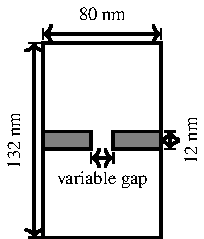
\includegraphics[width=\textwidth]{geometry_gap}
		%\tikzsetnextfilename{geometry_gap}
		%%\shorthandoff{:!}

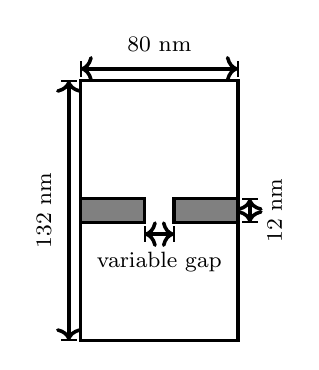
\begin{tikzpicture}[scale=0.025]

%%%%%%%%%%%%%%%%%%%%%%
%%%	 Def géométrie  %%%
%%%%%%%%%%%%%%%%%%%%%%

\def \diacnt{12}
\def \longueur{80}
\def \vspace{2}
\def \lignecote{8}
\def \hauteur{132}
\def \anglearc{111.5}
\def \gap{15}

%%%%%%%%%%%%%%%%%%%%%%
%%%	   Def style    %%%
%%%%%%%%%%%%%%%%%%%%%%

\def \heavy{0.045cm}
\def \light{0.025cm}

%%%%%%%%%%%%%%%%%%%%%%
%%%	    Calculs     %%%
%%%%%%%%%%%%%%%%%%%%%%

\pgfmathsetmacro{\sinangle}{sin(\anglearc)}
\pgfmathsetmacro{\cosangle}{cos(\anglearc)}

%%%%%%%%%%%%%%%%%%%%%%
%%%	    Dessin      %%%
%%%%%%%%%%%%%%%%%%%%%%

\draw[line width=\heavy] (0,0) rectangle (\longueur,\hauteur);
\draw[line width=\heavy, fill=gray] (0,0.5*\hauteur-0.5*\diacnt) rectangle (0.5*\longueur-0.5*\gap,0.5*\hauteur+0.5*\diacnt);
\draw[line width=\heavy, fill=gray] (0.5*\longueur+0.5*\gap,0.5*\hauteur-0.5*\diacnt) rectangle (\longueur,0.5*\hauteur+0.5*\diacnt);


%%%%%%%%%%%%%%%%%%%%%%
%%%	    Cotation    %%%
%%%%%%%%%%%%%%%%%%%%%%

% On dessine la ligne de cote pour l'espace entre les nanotubes
\draw[line width=\light] (0.5*\longueur-0.5*\gap,-\vspace+0.5*\hauteur-0.5*\diacnt) -- + (0,-\lignecote);
\draw[line width=\light] (0.5*\longueur+0.5*\gap,-\vspace+0.5*\hauteur-0.5*\diacnt) -- + (0,-\lignecote);
\draw[<->,line width=\heavy] (0.5*\longueur-0.5*\gap,-\vspace-0.5*\lignecote+0.5*\hauteur-0.5*\diacnt) -- + (\gap,0);

\node[anchor=north] (A) at (0.5*\longueur , -\vspace-\lignecote+0.5*\hauteur-0.5*\diacnt) {\footnotesize variable gap};

% On dessine la ligne de cote pour le diamètre des nanotubes
\draw[line width=\light] (\longueur+\vspace,0.5*\hauteur-0.5*\diacnt) -- + (\lignecote,0);
\draw[line width=\light] (\longueur+\vspace,0.5*\hauteur+0.5*\diacnt) -- + (\lignecote,0);
\draw[<->,line width=\heavy] (\longueur+\vspace+0.5*\lignecote,0.5*\hauteur-0.5*\diacnt) -- + (0,\diacnt);

\node[anchor=north, rotate=90] (B) at (\longueur+\vspace+\lignecote,0.5*\hauteur ) {\footnotesize \diacnt \ nm};

% On dessine la ligne de cote pour la hauteur
\draw[line width=\light] (-\vspace,0) -- + (-\lignecote,0);
\draw[line width=\light] (-\vspace,\hauteur) -- + (-\lignecote,0);
\draw[<->,line width=\heavy] (-\vspace-0.5*\lignecote,0) -- + (0,\hauteur);

\node[anchor=south, rotate=90] (C) at (-\vspace-\lignecote,0.5*\hauteur ) {\footnotesize \hauteur \ nm};

% On dessine la ligne de cote pour le diamètre du modèle
\draw[line width=\light] (0,\hauteur+\vspace) -- + (0,\lignecote);
\draw[line width=\light] (\longueur,\hauteur+\vspace) -- + (0,\lignecote);
\draw[<->,line width=\heavy] (0,\hauteur+\vspace+0.5*\lignecote) -- + (\longueur,0);

\node[anchor=south] (D) at (0.5*\longueur , \hauteur+\vspace+\lignecote) {\footnotesize \longueur \ nm};

%%%%%%%%%%%%%%%%%%%%%%%%%%%%%%%%%%%%%%%%%

\end{tikzpicture}

%\shorthandon{:!}
		%}
		\caption{Geometry of the third FEM simulating Joule heating within the polymer matrix}
		\label{fig:geometry_gap}
	\end{subfigure} 
	\caption{Geometries of the representative elementary volume composed of MWCNT (dark region) and the insulating matrix (white region) \cite{Brassard2018_figshare_article1}}
	\label{fig:geometry}
\end{figure}

\FloatBarrier

In the first model, a single MWCNT (Fig. \ref{fig:geometry_axisymmetric} dark zone), surrounded by PEI (Fig. \ref{fig:geometry_axisymmetric} white zone) was represented using axisymmetric boundary conditions. 
The top and bottom surfaces of the MWCNT acted as voltage source and ground, respectively, with the current flowing through the MWCNT. 
The diameter of the MWCNT was set to \SI{12}{\nano\metre} in agreement with the data obtained from our supplier. 
This model assumed heat generation through Joule effect inside the MWCNT and heat transfer by conduction occurring radially from the MWCNT to the polymer.

In the second model, the flow of the current has to cross through direct contact between adjacent nanotubes. 
The REV (Fig. \ref{fig:geometry_3D}) includes three MWCNTs (dark region) that form a percolated electrical path within the polymer matrix. 
The current from the voltage source must transfer through two contact point interfaces to reach the ground on the other side of the conductive network. 
The highlighted plane shows the area of interest for temperature monitoring. 
Joule heating from within the MWCNTs was also present in this model. 

In the third model, the current was forced to flow through a polymer gap, of variable length, between two adjacent MWCNTs (Fig. \ref{fig:geometry_gap}). 

In each simulation, a constant DC electric field was applied for \SI{5}{\second} and the resulting temperature field was recorded. 
The value of the electric field was adjusted so as to reach similar temperatures after \SI{5}{\second} in all three models. 
A volumetric electromagnetic heat source was used to simulate Joule heating. 
Conductive heat transfer within solids (Fourier's law) is considered and the current is conserved within the REV (conservation law). 
Electrical insulation and symmetric thermal boundary conditions were set for the edges of the polymer matrix that were not in contact with the MWCNT. 
Symmetric thermal boundary conditions were defined at both ends of the MWCNT. 
These boundary conditions were selected to simulate a REV far from the outer surfaces of the nanocomposite heating element. 
Under these conditions, heat was generated within the three models but had no way to exit, causing the temperature to increase as energy kept accumulating.

The physical properties of PEI were used for the polymer matrix alongside physical properties for MWCNT taken from the literature (Tab. \ref{tab:material_properties}). 

\begin{table}[h]
\center
\resizebox{\textwidth}{!}{
\begin{tabular}{@{}lllrlrl@{}}
\toprule
Property    					&                   &        												& PEI				&							& MWCNT 			& \\ \midrule
Density						& $\rho$            & [\si{\kilo\gram\per\cubic\metre}]  			& 1270 			&							& 2000 			& \cite{Lehman2011} \\
Specific heat				& $C_p$             & [\si{\joule\per\kilo\gram\per\celsius}] 	& 1248				& \cite{Ageorges2001}	& 600 				& \cite{Mizel99} \\
Thermal conductivity		& $k$               & [\si{\watt\per\metre\per\celsius}]  			& 0.22				&							& 3000				& \cite{Mizel99,Berber2000} \\
Electrical conductivity	& $\sigma$          & [\si{\siemens\per\metre}]    					& \num{1e-15} 	&							& \num{8.3e5}	& \cite{Ebbesen1996} \\
Relative permittivity		& $\upvarepsilon_r$ & [ \hspace{0.5em} ]												& 3.15  			&							& 12.5     		& \cite{Katsounaros2011} \\ \bottomrule
\end{tabular}}
\caption{Material properties, unless noted, the properties for PEI are taken from SABIC's technical documentation}
\label{tab:material_properties}
\end{table}

%%%%%%%%%%%%%%%%%%%%%%%%%%%%%%%%%%%%%%%%%%%%%%%%%%%%%%%%%%%%%%
\FloatBarrier
\subsection{Simulations Results}
%%%%%%%%%%%%%%%%%%%%%%%%%%%%%%%%%%%%%%%%%%%%%%%%%%%%%%%%%%%%%%

As expected, simulations from the first FEM show resistive heat generated only within the MWCNT (Fig. \ref{fig:heat_axysymmetric}). 
Current went through the conductive MWCNT and thermal conduction caused the heating of the polymer. 
A homogeneous temperature of \SI{200}{\celsius} is obtained for this simulation after \SI{5}{\second} under an electric field of \SI{100}{\volt\per\metre}. 

\begin{figure}[htb]
	\centering
	\captionsetup{width=\textwidth}
	\begin{subfigure}{0.49\textwidth}
		\centering
		\captionsetup{width=0.9\textwidth}
		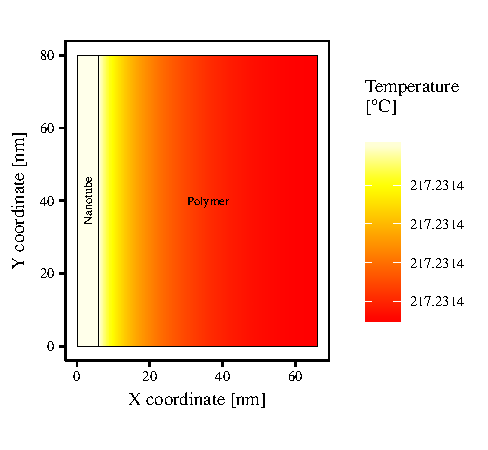
\includegraphics[width=\textwidth]{resultats_comsol_axisymetrique_temp}
		\caption{Uniform temperature field}
		\label{fig:temp_axysymmetric}
	\end{subfigure}
	\begin{subfigure}{0.49\textwidth}
		\centering
		\captionsetup{width=0.9\textwidth}
		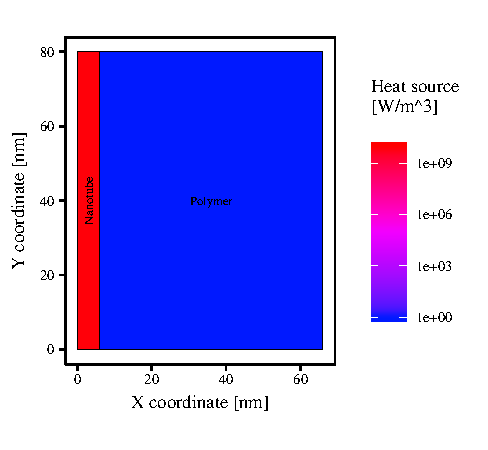
\includegraphics[width=\textwidth]{resultats_comsol_axisymetrique_puissance}
		\caption{Heat generation field}
		\label{fig:heat_axysymmetric}
	\end{subfigure}%	
	\caption{Results of the FEM evaluating the heat generation within the MWCNT. The uniform temperature field is due to the short time constant for thermal diffusion in the model (see section \ref{sec:timeconstant}). \cite{Brassard2018_figshare_article1}}
	\label{fig:results_axysymmetric}
\end{figure}

For the second FEM, the primary heat source was located at the contact point between the MWCNTs (Fig. \ref{fig:heat_3D}). 
Contribution from Joule heating within the MWCNTs was also present in the model with a power density 4 orders of magnitude lower. 
A uniform temperature profile is seen in MWCNTs, which is due to their high thermal conductivity. 
A uniform temperature of \SI{181}{\celsius} is obtained for this simulation after \SI{5}{\second} under an electric field of \SI{100}{\volt\per\metre}. 

\begin{figure}[htb]
	\centering
	\captionsetup{width=\textwidth}
	\begin{subfigure}{0.49\textwidth}
		\centering
		\captionsetup{width=0.9\textwidth}
		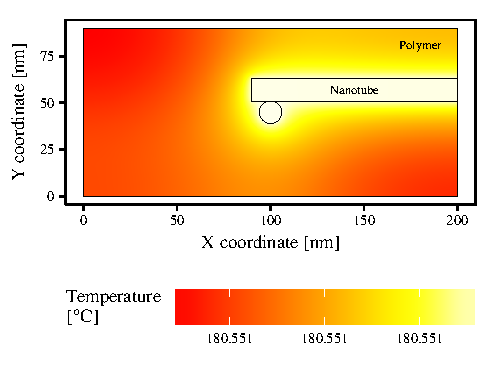
\includegraphics[width=\textwidth]{resultats_comsol_3D_temp}
		\caption{Uniform temperature field}
		\label{fig:temp_3D}
	\end{subfigure}
	\begin{subfigure}{0.49\textwidth}
		\centering
		\captionsetup{width=0.9\textwidth}
		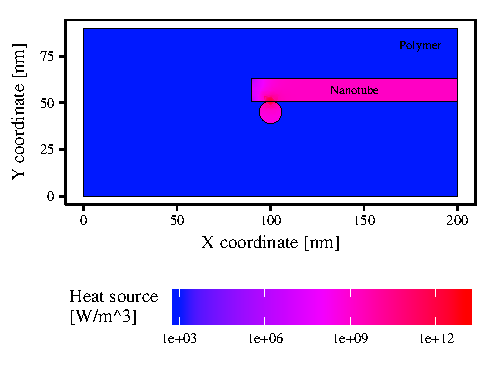
\includegraphics[width=\textwidth]{resultats_comsol_3D_puissance_log}
		\caption{Heat generation field}
		\label{fig:heat_3D}
	\end{subfigure}
	\caption{Results of the FEM evaluating the effect of charge concentration and contact resistance. The uniform temperature field is due to the short time constant for thermal diffusion in the model (see section \ref{sec:timeconstant}). \cite{Brassard2018_figshare_article1}}
	\label{fig:results_3D}
\end{figure}

\FloatBarrier

In the third FEM, heat generation occurred almost exclusively in the polymer matrix (Fig. \ref{fig:result_gap01nm_power} and \ref{fig:result_gap8nm_power}). 
Heat is generated in the bulk of the polymer and a uniform temperature profile is obtained in the model (Fig. \ref{fig:result_gap01nm_temp} and \ref{fig:result_gap8nm_temp}). 

The third model demonstrates that the electric field required to reach a temperature similar to that of the first two models increases sharply when a small gap is introduced in the conductive network (Fig. \ref{fig:result_gap}). 
A gap of \SI{0.1}{\nano\metre}, between adjacent MWCNTs, required a field of \SI{9e9}{\volt\per\metre} to produce a temperature of \SI{185}{\celsius} (Fig. \ref{fig:result_gap01nm_temp}). 
When the gap was increased to \SI{8}{\nano\metre} a field of \SI{5e10}{\volt\per\metre} was necessary to reach a similar temperature (Fig. \ref{fig:result_gap8nm_temp}). 
These electrical field intensities are superior to the dielectric strength of PEI (\SI{3.3e7}{\volt\per\metre}) and the current went through the bulk of the polymer matrix. 
That seven order of magnitude increase in the electrical field, when a gap is introduced, confirms that the third heating mode is unlikely in practical applications. 
A connected network of MWCNTs provides pathways of lower resistance for the electrons to flow. 
A sharp increase in the resistance is indicative of a perturbation in the percolated network. 

\begin{figure}[htb]
	\centering
	\begin{subfigure}{0.49\textwidth}
		\centering
		\captionsetup{width=0.9\textwidth}
		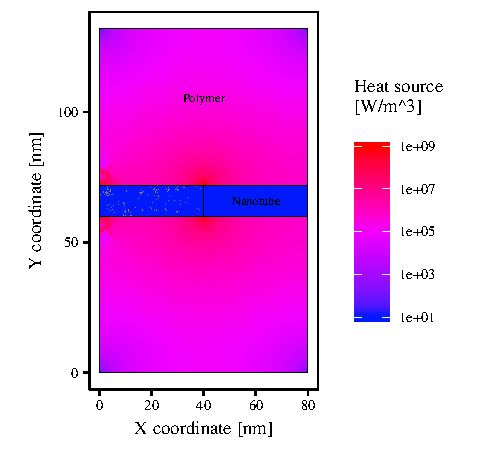
\includegraphics[width=\textwidth]{resultats_0,1nm_comsol_2D_puissance}
		\caption{\SI{0.1}{\nano\metre} gap, \SI{9e9}{\volt\per\metre}}
		\label{fig:result_gap01nm_power}		
	\end{subfigure} 
	\begin{subfigure}{0.49\textwidth}
		\centering
		\captionsetup{width=0.9\textwidth}
		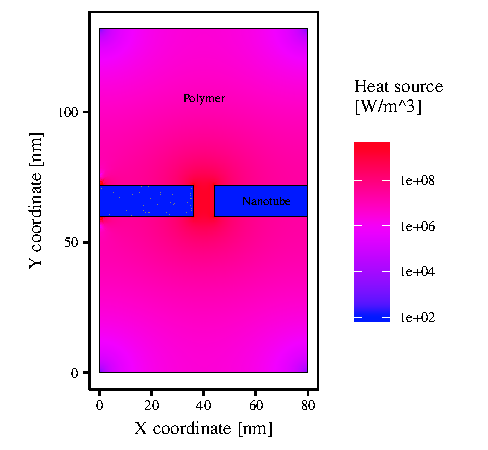
\includegraphics[width=\textwidth]{resultats_8nm_comsol_2D_puissance}
		\caption{\SI{8}{\nano\metre} gap, \SI{5e10}{\volt\per\metre}}
		\label{fig:result_gap8nm_power}		
	\end{subfigure}

	\begin{subfigure}{0.49\textwidth}
		\centering
		\captionsetup{width=0.9\textwidth}
		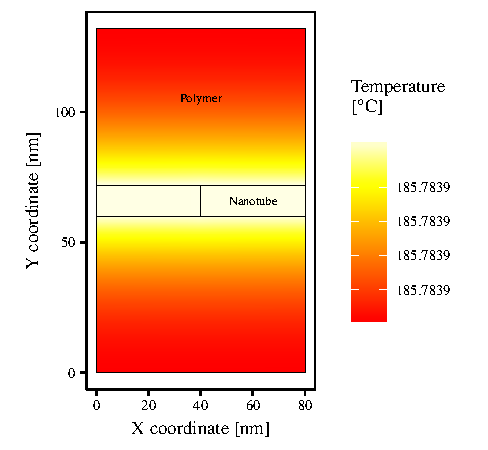
\includegraphics[width=\textwidth]{resultats_0,1nm_comsol_2D_temp}
		\caption{\SI{0.1}{\nano\metre} gap, \SI{9e9}{\volt\per\metre}}
		\label{fig:result_gap01nm_temp}		
	\end{subfigure} 
	\begin{subfigure}{0.49\textwidth}
		\centering
		\captionsetup{width=0.9\textwidth}
		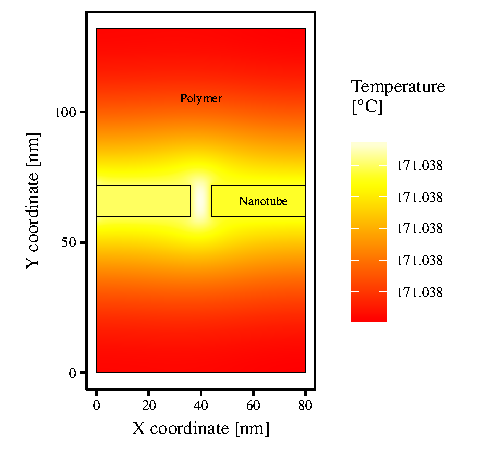
\includegraphics[width=\textwidth]{resultats_8nm_comsol_2D_temp}
		\caption{\SI{8}{\nano\metre} gap, \SI{5e10}{\volt\per\metre}}
		\label{fig:result_gap8nm_temp}		
	\end{subfigure}
	\caption{Effect of the gap length on the heat generation and temperature fields in the case of heat generation within the polymer. The uniform temperature fields are due to the short time constant for thermal diffusion in the model (see section \ref{sec:timeconstant}). \cite{Brassard2018_figshare_article1}}
	\label{fig:result_gap}
\end{figure}

From these results, we observe that conduction (and thus heat dissipation) within MWCNTs and through their contact points is the main driver for heat generation within a nanocomposite heating element. 
The uniform temperature fields observed at the constituent level lead to the conclusion that under normal operating conditions, local thermal degradation should not occur within the nanocomposite during the welding process. 

%%%%%%%%%%%%%%%%%%%%%%%%%%%%%%%%%%%%%%%%%%%%%%%%%%%%%%%%%%%%%%
\FloatBarrier
\subsection{Timescale analysis}
%%%%%%%%%%%%%%%%%%%%%%%%%%%%%%%%%%%%%%%%%%%%%%%%%%%%%%%%%%%%%%
\label{sec:timeconstant}

A comparative numerical analysis of the timescales for thermal diffusion, providing an explanation for the uniform temperature fields observed in the models, is presented in this section. 
Although PEI has poor thermal conductivity, uniform temperature fields with temperature variations not exceeding \SI{1e-5}{\celsius} are observed in the models. 
A comparative numerical analysis of the timescales for thermal diffusion, can explain this behaviour. 
This timescale is evaluated using the time constant for thermal diffusion ($t_D$) : 

\begin{equation}
	t_D = \frac{L^2}{\alpha}
	\label{equa:time_constant}
\end{equation}

\begin{figure}[htb]
	\center
	\captionsetup{width=35mm}
	%\resizebox{35mm}{!}{%\\
	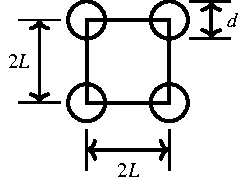
\includegraphics[width=35mm]{arrangement_carre}
	%\tikzsetnextfilename{arrangement_carre}
	%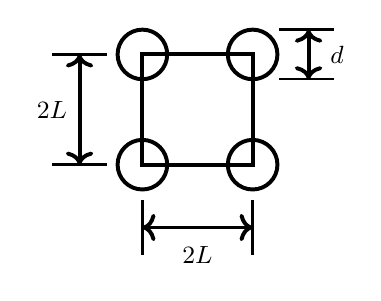
\begin{tikzpicture}[scale=1.4]

\def \l{1}
\def \r{0.225}
\def \vspace{0.32}
\def \lignecote{0.5}

\def \heavy{0.05cm}
\def \light{0.03cm}

\draw[line width=\heavy] (0,0) rectangle (\l,\l);

\draw[line width=\heavy] (0,0) circle (\r);
\draw[line width=\heavy] (\l,0) circle (\r);
\draw[line width=\heavy] (0,\l) circle (\r);
\draw[line width=\heavy] (\l,\l) circle (\r);

\draw[line width=\light] (0,-\vspace) -- + (0,-\lignecote);
\draw[line width=\light] (\l,-\vspace) -- + (0,-\lignecote);
\draw[<->,line width=\heavy] (0,-\vspace-0.5*\lignecote) -- + (\l,0);

\node (A) at (0.5*\l , -\vspace-\lignecote) {\small $2L$};

\draw[line width=\light] (-\vspace,0) -- + (-\lignecote,0);
\draw[line width=\light] (-\vspace,\l) -- + (-\lignecote,0);
\draw[<->,line width=\heavy] (-\vspace-0.5*\lignecote,0) -- + (0,\l);

\node (A) at (-\vspace-\lignecote,0.5*\l ) {\small $2L$};

\draw[line width=\light] (\l+0.75*\vspace,\l-\r) -- + (\lignecote,0);
\draw[line width=\light] (\l+0.75*\vspace,\l+\r) -- + (\lignecote,0);
\draw[<->,line width=\heavy] (\l+\vspace+0.375*\lignecote,\l-\r) -- + (0,2*\r);

\node (A) at (\l+\vspace+0.25*\lignecote+\vspace,\l ) {\small $d$};


\end{tikzpicture}
	%}
	\caption{Square packing micromechanic model \cite{Brassard2018_figshare_article1}}
	\label{fig:square_packing}
\end{figure}

Assuming a uniform square packing of evenly distributed particles (Fig. \ref{fig:square_packing}) of known diameter ($d$) and variable volume fractions ($v_f$), it is possible to evaluate the average half distance ($L$) between particles :

\begin{equation}
	L = \sqrt{\frac{\pi \ d^2}{16 \ v_f}}
	\label{equa:L_average}
\end{equation}

The thermal diffusivity ($\alpha$) is defined as a function of thermal conductivity ($k$), density ($\rho$) and specific heat ($C_p$) : 

\begin{equation}
	\alpha = \frac{k}{\rho \ C_p}
	\label{equa:thermal_diffusivity}
\end{equation}

\begin{table}[htb]
\centering
%\resizebox{88mm}{!}{
\begin{tabular}{@{}p{2.6cm}p{2.7cm}p{2.2cm}p{1.7cm}@{}}
%\begin{tabular}{@{}llll@{}}
\toprule
Weight fraction of MWCNTs	& Volume fraction of MWCNT	& Average half distance 	& \textbf{Time constant}  		\\ %\midrule
$w_f$								& $v_f$ 							& L 							& $\mathbf{t_D}$            	\\
{[}\%{]}							& {[}\%{]	}						& {[}nm{]} 					& \textbf{{[}s{]}}            	\\ \midrule
1									& 0.65 							& 65.8	 						& $\mathbf{3\times 10^{-8}}$ 	\\ 
5									& 3.31								& 29.2							& $\mathbf{6\times 10^{-9}}$	\\
10									& 6.74								& 20.5							& $\mathbf{3\times 10^{-9}}$	\\
16									& 11.02 							& 16.0 						& $\mathbf{2\times 10^{-9}}$	\\	\bottomrule
\end{tabular}%}
\caption{Timescale for heat conduction}
\label{tab:results_timescale}
\end{table}

Since the thermal conductivity of MWCNTs is very high compared to the polymer, only the properties of the matrix were considered in this timescale analysis. 
Table \ref{tab:results_timescale} presents the time constants calculated for thermal diffusion within the polymer matrix. 
The time constants varied from $3 \times 10^{-8}$ to \SI{2e-9}{\second} for $v_f$ varying from 1\% to 16\%. 
Considering that the simulations looked at Joule heating on a scale closer to the second, the short timescales for thermal diffusion explain the constant temperature fields. 

%%%%%%%%%%%%%%%%%%%%%%%%%%%%%%%%%%%%%%%%%%%%%%%%%%%%%%%%%%%%%%
\subsection{FTIR results}
\FloatBarrier
%%%%%%%%%%%%%%%%%%%%%%%%%%%%%%%%%%%%%%%%%%%%%%%%%%%%%%%%%%%%%%

We collected FTIR spectra from a virgin PEI pellet, a nanocomposite PEI/MWCNT pellet, a nanocomposite film and two spectra from a fracture surface of a welded zone. 
The resulting absorbances spectra were calculated. 
The appearance of characteristic peaks, their position and width remained the same between the different spectra. 

\begin{figure}[h]
	\center
	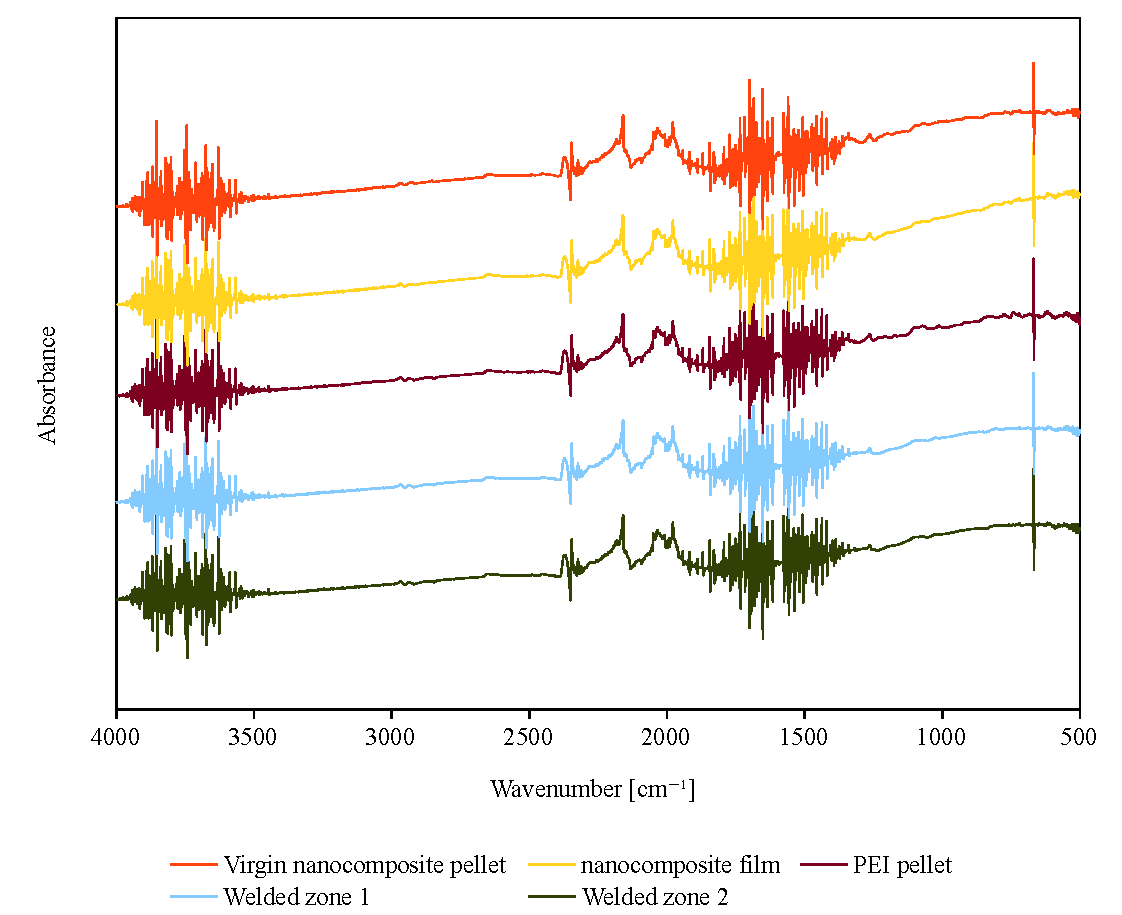
\includegraphics[width=\textwidth]{FTIR_spectra.pdf}
	\caption{Raw FTIR spectra \cite{Brassard2018_figshare_article1}}
	\label{fig:FTIR_spectra}
\end{figure}



\FloatBarrier
%%%%%%%%%%%%%%%%%%%%%%%%%%%%%%%%%%%%%%%%%%%%%%%%%%%%%%%%%%%%%%%%%
							\section{References}
%%%%%%%%%%%%%%%%%%%%%%%%%%%%%%%%%%%%%%%%%%%%%%%%%%%%%%%%%%%%%%%%%

\bibliographystyle{plainnat}
\bibliography{Article_soudage_nano_1}
%\pagebreak

%\section{Figures}
%\FloatBarrier
\end{document}
